\chapter{Time discretization and optimalization}

The aim of this chapter is to present some of the main challenges regarding discretization of a general monolithic fluid-structure interaction(FSI) problem, using the ALE-framework. Even separately, the discretization of fluid and structure problems impose rather difficult issues due to their non-linear nature. However, their long-time existence within research community makes them well known problems and a vast number of rigorous approaches and commercial  software exist to solve them individually. When solving the fluid and structure simultaneously however, the overall problem gets more complex due to the overall dependency of the two sub-problems and their interaction to one another. 

One of the main challenges is the additional non-linearty intruduced by the domain-velocity term in the fluid problem. 
\begin{prob}
\textit{ALE term}\begin{align*}
\ha{J} (\hat{F}_W^{-1}(\bat{v} - \pder{\ha{T}_W}{t}) \cdot \hat{\nabla}) \bat{v}
\end{align*} 
\end{prob}
Closer inspection of the convection term reviels spatial and temporal differential operators depending non-linearly on one another. Within computational science, these operators often appear separated. Therefore the discretization of a general time-stepping scheme  is not directly intuitive, and often based on the experience of similar equations such as the Navier-Stokes equations. In this thesis, time-stepping schemes of second order will be considered.
It has been reported in [] [], that the stability of first and second-order time stepping schemes are affected by the ALE-convection term, but to what extent remains unclear.\\
Though only the fluid problem will be discussed, it must be emphasized that the discretization of the solid problem is of great importance. Several studies exists for the individual solid problem, but a deeper analysis considering a fluid-structure interaction setting is abvient from the FSI litterature \cite{Richter2015}.                                                                                                                                                                                                                       




\section{Implementation of a one-step $\theta$ scheme} 
For both the fluid problem and the structure problem, we will base our implementation of a $\theta$-scheme.  A $\theta$-scheme is favourable, making implementation of classical time-steppings schemes simple. For the structure problem,  $\theta$-scheme takes the form

\begin{prob}
\begin{align*}
\rho_s \pder{\bat{v}_s}{t} 
- \theta \nabla \cdot \bat{F}\bat{S}   - (1 - \theta) \nabla \cdot \bat{F}\bat{S}  
- \theta \rho_s \bat{f}_s 
- (1 - \theta) \rho_s \bat{f}_s = 0 \\
\pder{\bat{v}_s}{t} - \theta \bat{u}_s - (1 - \theta)\bat{u}_s  = 0&\\
\end{align*} 
\end{prob}

For $\theta \in [0, 1]$ classical time-stepping schemes are obtained such as the first-order forward Euler scheme $\theta = 0$, backward-Euler scheme$\theta = 1$, and the second-order Crank-Nicholson scheme $\theta = \frac{1}{2}$.  \\

Studying the fluid problem, it is initially simpler to consider the Navier-Stokes equation in an Eulerian formulation rather the ALE-formulation Following \cite{Simo1994}, a general time stepping algorithm for the coupled Navier-Stokes equation can be written as

\begin{prob}
\begin{align*}
\frac{1}{\Delta}(\mathbf{u}^{n+1} - \mathbf{u}^{n}) + 
B(\mathbf{u}^{*})\mathbf{u}^{n+\alpha}
- \nu \nabla^2 \mathbf{u}^{n + \alpha} = - \nabla p + \mathbf{u}^{n+\alpha} \\
\nabla \cdot \mathbf{u}^{n+\alpha} = 0 
\end{align*} 
\end{prob}

Here $\mathbf{u}^{n+\alpha}$ is an "intermediate" velocity defined by,
\begin{align*}
\mathbf{u}^{n+\alpha} = \alpha\mathbf{u}^{n+1} + (1 - \alpha)\mathbf{u}^{n} 
\hspace{4mm} \alpha \in [0, 1]
\end{align*}
while $\mathbf{u}^{*}$ is on the form

\begin{align*}
\mathbf{u}^{*} =   \mathbf{u}^{n+ \vartheta} =
\begin{cases} 
   &\vartheta \mathbf{u}^{n+1} + (1 - \vartheta)\mathbf{u}^{n} \hspace{4mm} \vartheta \geq 0 \\ 
   &\vartheta \mathbf{u}^{n-1} + (1 - \vartheta)\mathbf{u}^{n} \hspace{4mm} \vartheta \leq 0
   \end{cases}
\end{align*}
At first glance, defining an additional parameter $\vartheta$ for the fluid problem seems unessecary. A general mid-point rule by  $\alpha = \vartheta = \frac{1}{2}$, a second order scheme in time would easily be acchieved. However, in \cite{Simo1994} an additional second order scheme is obtained by choosing e $\alpha = \frac{1}{2}$,  $\vartheta =-1$, where  $\mathbf{u}^{*}$ is approximated with an Adam-Bashforth linear method. Making the initial fluid problem linear while maintaining second order convergence is an important result, which have not yet been investigated thorough in litterature of fluid-structure interaction. One reason for this may be that the ALE fluid problem will remain non-linear due to the ALE-mapping.

 
For the structure problem, the Crank-Nicholson is of main interest due to energy preservation properties and second order convergence. \\


In light of By letting $\alpha = \vartheta \hspace{2mm} \alpha, \vartheta \in [0, 1] $ for the fluid problem, and generalising the consepts in an ALE context, we derive the one-stepl $\theta$ scheme found in \cite{Wicka}.

\begin{prob}
\textit{One-step $\theta$-scheme for laplace and elastic mesh moving model.
Find $\bat{u}_s, \bat{u}_f, \bat{v}_s, \bat{v}_f, \ha{p}_f $ such that}
\begin{align*}
\big(\ha{J}^{n, \theta} \pder{\bat{v}}{t}, \ \gat{\psi}^u \big)_{\hat{\Omega}_f} +
\theta \femf{\ha{J} \hat{F}_W^{-1}(\bat{v} \cdot \hat{\nabla}) \bat{v}}
{\gat{\psi}^u} + 
(1 - \theta) \femf{\ha{J} \hat{F}_W^{-1}(\bat{v} \cdot \hat{\nabla}) \bat{v}}
{\gat{\psi}^u} \\
- \femf{\ha{J}  \pder{\ha{T}_W}{t} \cdot \hat{\nabla}) \bat{v}}
{\gat{\psi}^u}
-\theta \femf{\ha{J}_W \hat{\sigma}\hat{F}_W^{-T}}{\hat{\nabla}\gat{\psi}^u} -
- (1 - \theta) \femf{\ha{J}_W \hat{\sigma}\hat{F}_W^{-T}}{\hat{\nabla}\gat{\psi}^u} \\
- \theta \femf{\rho_f \ha{J} \mathbf{f}_f}{{\gat{\psi}^u}} - 
(1 - \theta) \femf{\rho_f \ha{J} \mathbf{f}_f}{{\gat{\psi}^u}}= 0& \\
\fems{\rho_s \pder{\bat{v}_s}{t}}{\gat{\psi}^u} + 
- \theta\fems{\bat{F}\bat{S}}{\nabla \gat{\psi}^u}  + 
- (1 - \theta) \fems{\bat{F}\bat{S}}{\nabla \gat{\psi}^u} \\
- \theta \fems{\rho_s \bat{f}_s}{\gat{\psi}^u} 
- (1 - \theta) \fems{\rho_s \bat{f}_s}{\gat{\psi}^u} = 0 \\
\fems{\pder{\bat{v}_s}{t} - \theta \bat{u}_s - (1 - \theta)\bat{u}_s}{\gat{\psi}^v}  = 0&\\
\femf{\nabla \cdot (\ha{J} \hat{F}_W^{-1} \bat{v})}{\gat{\psi}^p} = 0& \\
\femf{\hat{\sigma}_{\text{mesh}}}{\hat{\nabla}\gat{\psi}^u} = 0&
\end{align*} 
\end{prob}

Deeper analysis in  \cite{Wicka}, specify to important properties of the one-step $theta$ scheme. Firstly, it is unconditionally stable regardless of time step for the interval $\theta = [\frac{1}{2}, 1]$. 

\subsection{Temporal stability}
It is known that the Crank-Nicolson scheme can suffer from temporal stability, for long-term simulations \cite{Wick2013a}.

Preliminary work regarding discretization and numerical analysis of Crank-Nicholson time stepping schemes for fluid structure interaction can be found in cite WIck papers. Two main properties of interest of higher-order methods have proven to be the stability of long-time simulation, and obtaining the expected physics for the problem of interest.

The authors of \cite{Richter2015}, investigated temporal stability of the Crank-Nicolson scheme for the validation benchmark found in \cite{Hron2006}.  
The critera for the numerical experiements was to obatin a stable solution in the time interval [0, 10] minutes, by temporal and spatial refinement studies. The fully monolithic FSI problem discretized with second-order Crank-Nicolson, proved to give general stability problems for long-term simulation. 

Following the ideas of Rick, whricter, a second order scheme based on the Cranck-Nicholson yields two possibilities.
\begin{discr}
\textit{Crank–Nicolson secant method }
\begin{align*}
\Big[\frac{\ha{J}(\bat{u}^{n}) \bat{\nabla} \bat{v}^{n} \bat{F}_W^{-1}}{2} 
+ \frac{\ha{J}(\bat{u}^{n-1}) \bat{\nabla} \bat{}v^{n-1} \bat{F}_W^{-1}}{2} \Big] 
\frac{\bat{u}^{n} - \bat{u}^{n-1}}{k}
\end{align*} 
\end{discr}

\begin{discr}
\textit{Crank–Nicolson midpoint-tangent method}
\begin{align*}
\Big[\frac{\ha{J}(\bat{u}_{cn}) \bat{\nabla} \bat{v}_{cn} \bat{F}_W^{-1}}{2} \Big] 
\frac{\bat{u}^{n} - \bat{u}^{n-1}}{k} \hspace{4mm}
\bat{u}_{cn} = \frac{\bat{u}^{n} + \bat{u}^{n-1}}{2} \hspace{2mm}
\bat{v}_{cn} = \frac{\bat{v}^{n} + \bat{v}^{n-1}}{2}
\end{align*} 
\end{discr}

The numerical experiments showed very similar performance for Discretization 1.1 and 1.2 , and significant differences of temporal accuracy was not found. \\
Two options to coupe with the presented unstabilities are the \textit{shifted Crank-Nicolson} \cite{Richter2015}, \cite{Wicka}, \cite{Wick2013a},   and the \textit{frac-step method}. Both of these methods are defined as A-stable time-stepping schemes meaning..  In this thesis the shifted Crank-Nocolson scheme will be considered. \\
The shifted Crank-Nicolson scheme introduce further stability to the overall system, by shifting the $\theta$ paramter slightly to the implicit side. If the shift is dependent of the time-step size, the scheme will be of second order \cite{Richter2015}.





\section{Optimization of Newtonsolver}
The expression \textit{bottleneck} esxpress a phenomen where the total performance of a complete implementation is limited to small code fragments, accounting for the primary consumption of computer resources.

As for many other applications, within computational science one can often assume the consummation of resources follows the \textit{The Pareto principle}. Meaning that for different types of events, roughly 80\% of the effects come from 20\% of the causes. An analogy to computational sciences it that 80\% of the computational demanding operations comes from 20\% of the code. In our case, the bottleneck is the newtonsolver. The two main reasons for this is 

\begin{itemize}
\item \textbf{Jacobian assembly} \\
The construction of the Jacobian matrix for the total residue of the system, is the most time demanding operations within the whole computation. 
\item \textbf{Solver}. \\ 
As iterative solvers are limited for the solving of fluid-structure interaction problems, direct solvers was implemented for this thesis. As such, the operation of solving a linear problem at each iteration is computational demanding, leading to  less computational efficient operations. Mention order of iterations?
\end{itemize}

Facing these problems, several attempts was made to speed-up the implementation. The FEniCS project consist of several nonlinear solver backends, were fully user-customization option are available. However one main problem which we met was the fact that FEniCS assembles the matrix of the different variables over the whole mesh, even though the variable is only defined in one to the sub-domains of the system.In our case the pressure is only defined within the fluid domain, and therefore the matrix for the total residual consisted of several zero columns within the structure region. FEniCS provides a solution for such problems, but therefore we were forced to construct our own solver and not make use of the built-in nonlinear solvers. \\

The main effort of speed-up were explored around the Jacobian assembly, as this was within our control.  

Of the speed-ups methods explored in this thesis we will specify that some of them were \textit{consistent} while others were \textit{nonconsistent}. Consistent methods are methods that always will work, involving smarter use of properties regarding the linear system to be solved. The non-consistent method presented involves altering the equation to be solved by some simplification of the system. As these simplifications will alter the expected convergence of the solver, one must take account for additional Newton iterations against cheaper Jacobi assembly. Therefore one also risk breakdown of the solver as the Newton iterations may not converge.   


\section{Consistent methods}
\subsection{Jacobi buffering}
By inspection of the Jacobi matrix, some terms of the total residue is linear terms, and remain constant within each time step. By assembling these terms only in the first Newton iteration will save some assembly time for the additional iterations needed each time step. As consequence the convergence of the Newton method should be unaffected as we do not alter the system.  

\section{Non-consisten methods}    
\subsection{Reuse of Jacobian}
As the assembly of the Jacobian at each iteration is costly, one approach of reusing the Jacobian for the linear system was proposed. In other words, the LU-factorization of the system is reused until the Jacobi is re-assembled. This method greatly reduced the computational time for each time step. By a user defined parameter, the number of iterations before a new assembly of the Jacobian matrix can be controlled. 

\subsection{Quadrature reduce}
The assemble time of the Jacobian greatly depends on the degree of polynomials used in the discretisation of the total residual. Within FEniCS this parameter can be controlled, and as such we can specify the order of polynomials representing the Jacobian. The use of lower order polynomials reduces assemble time of the matrix at each newton-iteration, however it leads to an inexact Jacobian which may results to additional iterations. 


\begin{figure}[h!]
\hspace*{-2.2cm}   
 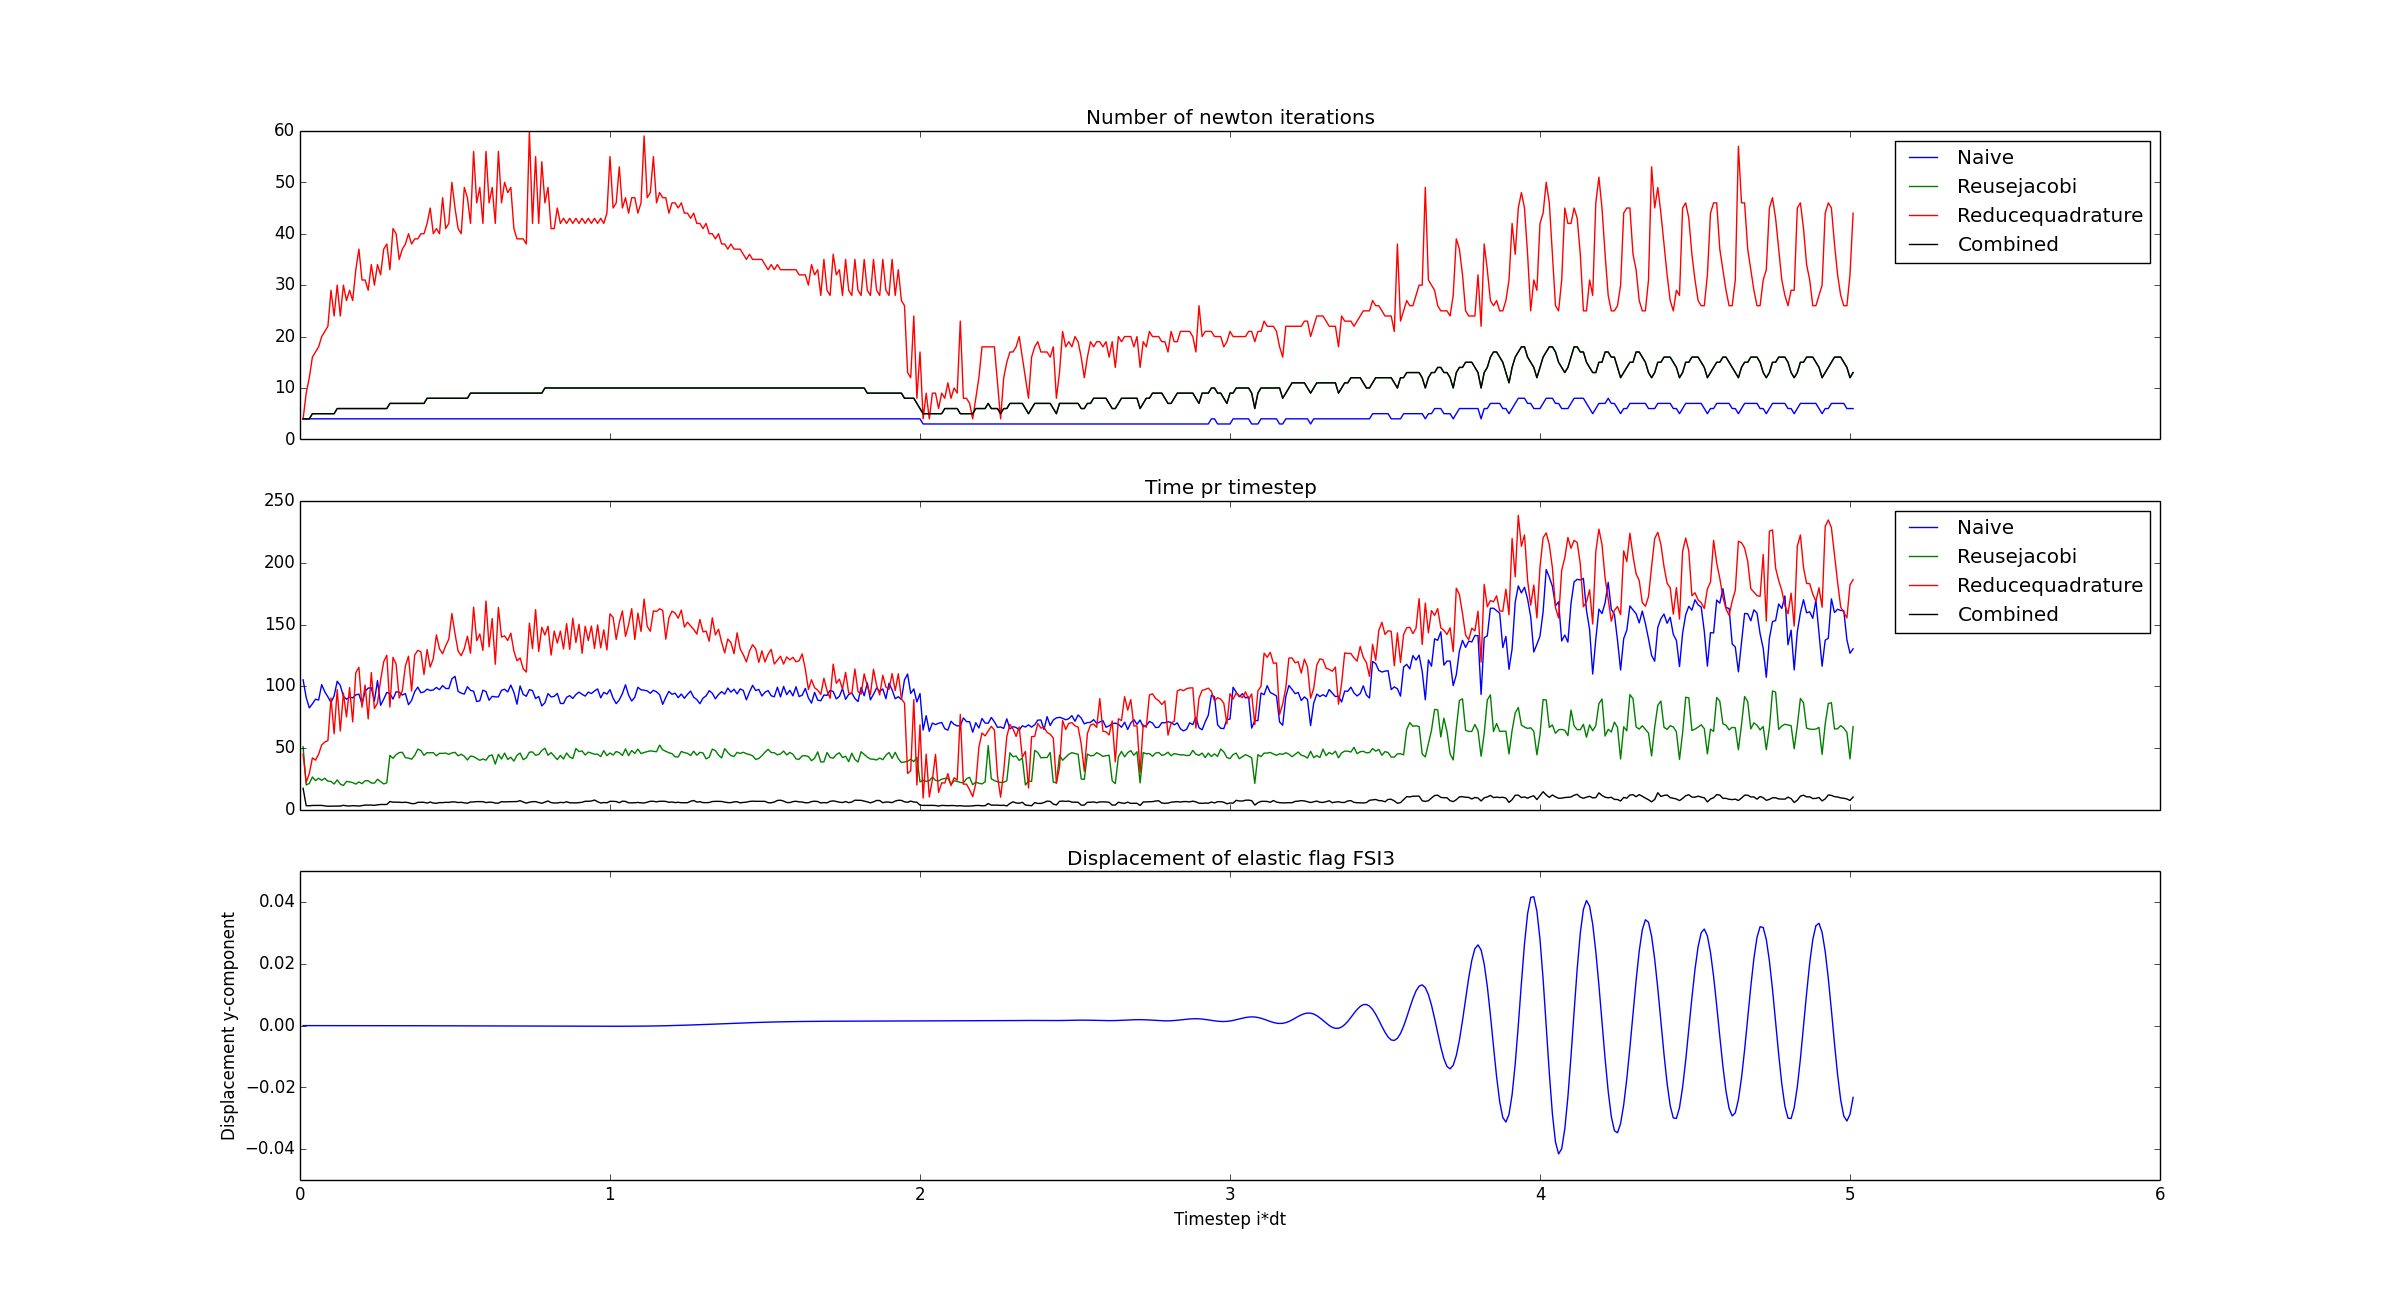
\includegraphics[scale=0.36]{./Fig/itercompare.png}
 \caption{Computational domain of the validation benchmark}
\end{figure}

\begin{table}[h]
\centering
\caption{Comparison of speedup techniques }
\label{my-label}
\begin{tabular}{ |p{2.8cm}|p{2.4cm}||p{2.4cm}|p{2.4cm}|p{2.4cm}|  }
 %\hline
 %\multicolumn{4}{|c|}{Solid parameters} \\
 \hline
Implementation &Naive  & Reducequad. & Reusejacobi & Combined \\
 \hline
 Mean time/timestep &   104.5 &  125.5 & 48.3  & 6.8   \\
 \hline
 Speedup & 1.0 &  1.20  & 0.46  & 0.06   \\
 \hline
 Mean iteration &  4.49 &  30.59 & 10.29  & 10.29   \\
 \hline
\end{tabular}
\end{table}

\newpage
A brief description will be given for the most central components and technologies used for this thesis. 

\newpage